\chapter{Metodología propuesta}\label{cap:propuesta}

En este capítulo se describe el marco metodológico de este trabajo, se explicará de manera explicita como es que cada uno de los componentes usados funciona.\\

Explicaremos los \textit{schemas} de la base de datos utilizados dónde se encuentran las tablas destinadas a usarse para los tableros de datos, entre estas se encuentran tablas con datos de ingresos, egresos, traslados, defunciones e información de cada paciente. Se hablará de la información que almacena cada tabla y como se relaciona cada tabla con las demás.\\

Se describirá brevemente como está organizada la arquitectura de la aplicación web dónde el trabajo realizado fue implementado. También, se mostrará un mockup proporcionado por \textbf{SEDESA} par ser tomado de base para su implementación en la parte del Frontend.\\

Se explicará la manera en que se desarrollaron los endpoints en el Backend mediante Django, su módelo de vistas (\textit{Views}) y con el apoyo de las bibliotecas de manejo de datos: NumPy y Pandas.\\

Por último, se abordará como implementó la parte visual del Frontend mediante la llamada de endpoints y los módulos de ReactJS para la visualización de datos usando la biblioteca de AmCharts.



\section{Base de datos}\label{sec:bd}
% - Mencionar que la información se importa a nuestra BD mediante un proceso de ETL (que esto no forma parte de este proyecto.)
% -Explicar las tablas de el esquema de tableros.

Como se ha venido mencionando en los capítulos anteriores, la base de datos está en implementada en PostgreSQL.\\
En la base de datos podemos encontrar diferentes \textit{schemas}: general, dashboards, medicalrecord, public y triage. Cada una de las tablas contenida en los schemas son pobladas mediante un proceso ETL desarrollado en script de Python. El proceso ETL recibe los datos a través de un archivo con extensión \textit{xls} que es obtenido a través del SAMI. Sin embargo, el desarrollo e implementación del proceso ETL queda fuera del contexto de este trabajo.\\

En particular los \textit{schemas} utilizado para este trabajo son \textbf{dashboards}, \textbf{triage} y \textbf{general}.
\newpage

A continuación se describirá cada una de las tablas utlizadas para realizar las consultas necesarias para el tablero de datos.

\begin{itemize}
    \item \textbf{general}
        \begin{itemize}
            \item \texttt{thospital}\\
            Una tabla de dimensión que almacena información de los hospitales pertenecientes a SEDESA. Es usada para realizar \textit{JOINs} en consultas dónde se requiera obtener información de hospitales.

            La columnas que conforman la tablas son las siguientes:

            \begin{itemize}
                \item \texttt{thospital\_id: integer} - Identificador único de cada hospital. Es la llave primaria.
                
                \item \texttt{nombre: CHARVAR} - El nombre completo del hospital.
            
                \item \texttt{nombre\_corto: CHARVAR} - El nombre corto con el que el hospital es identificado.
                
                \item \texttt{direccion: CHARVAR} - La dirección en la que el hospital se encuentra.
                \item \texttt{atiende\_covid19: boolean} - Columna para indicar si el hospital atiende paciente contagiagos de COVID-19
                \item \texttt{clues: CHARVAR} - La clave correspondiente al el Catálogo de Clave Unica de Establecimientos en Salud (CLUES).
                \item \texttt{cp: integer} - El código postal correspondiente al hospital.
            \end{itemize}


            
        \end{itemize}


    \item \textbf{triage}
    \begin{itemize}
        \item \texttt{cantecendete}\\
        Una tabla de dimensión que almacena información de diversas enfermedades.\\

        Las columnas que contiene son las siguientes:
        \begin{itemize}
            \item \texttt{cantecedente\_id: integer} - Identificador único del antecedente.
            
            \item \texttt{cantecedente\_primario\_id: integer} - Identificador del antecedente (enfermedad) primario.
            
            \item \texttt{nombre: CHARVAR} - Nombre del antecedente.
            
            \item \texttt{abreviatura: CHARVAR} - Abreviatura del antecedente.
            
            \item \texttt{sinonimos: CHARVAR} - Sinónimos asociados al antecedente.
            
            \item \texttt{triage: boolean} - Indica si el antecedente se utiliza en el triage.
        \end{itemize}

    \end{itemize}
        
    
    \item \textbf{dashboards}
        \begin{itemize}
            \item \texttt{tpaciente\_sami}

            Esta es una tabla de de dimensión, la cual contiene información personal de los pacientes hospitalizados. \\

            Las columnas que contiene son las siguientes: 

            \begin{itemize}
                \item \texttt{tpaciente\_sami\_id: integer} - Identificador único del paciente en el sistema SAMI.
                
                \item \texttt{fecha\_nacimiento: date} - Fecha de nacimiento del paciente.
                
                \item \texttt{indigena: boolean} - Indica si el paciente es de origen indígena.
                
                \item \texttt{calle: CHARVAR} - Nombre de la calle de residencia del paciente.
                
                \item \texttt{colonia: CHARVAR} - Nombre de la colonia de residencia del paciente.
                
                \item \texttt{codigo\_postal: integer} - Código postal de la residencia del paciente.
                
                \item \texttt{entidad\_federativa: CHARVAR} - Entidad federativa de residencia del paciente.
                
                \item \texttt{nombre: CHARVAR} - Nombre del paciente.
                
                \item \texttt{apellido\_paterno: CHARVAR} - Apellido paterno del paciente.
                
                \item \texttt{apellido\_materno: CHARVAR} - Apellido materno del paciente.
                
                \item \texttt{sexo: character} - Género del paciente.
                
                \item \texttt{estado: CHARVAR} - Estado de la república dónde reside el paciente.
                
                \item \texttt{municipio\_alcaldia: CHARVAR} - Municipio o alcaldía de residencia del paciente.
                
                \item \texttt{curp: CHARVAR} - Clave Única de Registro de Población del paciente.
                
                \item \texttt{codigo\_chn: integer} - Código correspondiente en el sistema CHN.
            \end{itemize}


            
            \item \texttt{tingreso\_paciente}

            Una tabla de hechos que almacena todos los ingresos de los pacientes a los hospitales.\\

            Las columnas que contiene son las siguientes:
            \begin{itemize}
                \item \texttt{tingreso\_paciente\_id: integer} - Identificador único de ingreso del paciente.
                
                \item \texttt{dosis\_covid: CHARVAR} - Información sobre las dosis de la vacuna contra COVID-19 con la que el paciente ha sido vacunado.
                
                \item \texttt{edad: integer} - Edad del paciente.
                
                \item \texttt{resultado\_prueba: CHARVAR} - Resultado de la prueba realizada al paciente.
                
                \item \texttt{ventilador: boolean} - Indica si el paciente requiere ventilador.
                
                \item \texttt{chn: integer} - Identificador en el sistema CHN.
                
                \item \texttt{fecha\_ingreso: timestamp} - Fecha y hora de ingreso del paciente.
                
                \item \texttt{diagnostico\_respiratorio: CHARVAR} - Diagnóstico respiratorio del paciente.
                
                \item \texttt{peso: numeric} - Peso del paciente.
                
                \item \texttt{talla: integer} - Talla del paciente.
                
                \item \texttt{imc: numeric} - Índice de masa corporal del paciente.
                
                \item \texttt{temperatura: numeric} - Temperatura del paciente.
                
                \item \texttt{tpaciente\_sami\_id: integer} - Identificador único del paciente en el sistema SAMI.
                
                \item \texttt{tetl\_reporte\_historico\_id: integer} - Identificador histórico del reporte en el sistema ETL.
                
                \item \texttt{thospital\_id: integer} - Identificador único del hospital.
                
                \item \texttt{servicio\_actual\_id: integer} - Identificador del servicio actual del paciente.
                
                \item \texttt{servicio\_ingreso\_id: integer} - Identificador del servicio al momento del ingreso del paciente.
                
                \item \texttt{seccion\_ingreso\_id: integer} - Identificador de la sección al momento del ingreso del paciente.
                
                \item \texttt{seccion\_actual\_id: integer} - Identificador de la sección actual del paciente.
                
                \item \texttt{vacunado\_covid: boolean} - Indica si el paciente ha sido vacunado contra COVID-19.
            \end{itemize}
            
            \item \texttt{tegreso\_paciente}

            Una tabla de hechos que almacena todos los egresos de los pacientes en los hospitales.\\

            Las columnas que contiene son las siguientes:
            \begin{itemize}
                \item \texttt{tegreso\_paciente\_id: integer} - Identificador único de egreso del paciente.
                
                \item \texttt{prueba\_confirmatoria: boolean} - Indica si se realizó una prueba confirmatoria.
                
                \item \texttt{resultado\_prueba: CHARVAR} - Resultado de la prueba realizada al paciente.
                
                \item \texttt{ventilador: boolean} - Indica si el paciente requiere ventilador.
                
                \item \texttt{diagnostico\_respiratorio: CHARVAR} - Diagnóstico respiratorio del paciente.
                
                \item \texttt{fecha\_alta: date} - Fecha de alta del paciente.
                
                \item \texttt{cmotivo\_alta\_id: integer} - Identificador del motivo de alta.
                
                \item \texttt{tpaciente\_sami\_id: integer} - Identificador único del paciente en el sistema SAMI.
                
                \item \texttt{tetl\_reporte\_historico\_id: integer} - Identificador histórico del reporte en el sistema ETL.
                
                \item \texttt{seccion\_egreso\_id: integer} - Identificador de la sección al momento del egreso del paciente.
                
                \item \texttt{servicio\_egreso\_id: integer} - Identificador del servicio al momento del egreso del paciente.
            \end{itemize}
            
            
            \item \texttt{tcomorbilidad\_ingreso}\\
            Una tabla de hechos que almacena la comorbilidad con la que ingreso un paciente.\\

            Las columnas que contiene son las siguientes:
            \begin{itemize}
                \item \texttt{tcomorbilidad\_ingreso\_id: integer} - Identificador único de la comorbilidad de ingreso.
                
                \item \texttt{tingreso\_paciente\_id: integer} - Identificador único de ingreso del paciente.
                
                \item \texttt{cantecedente\_id: integer} - Identificador único del antecedente asociado a la comorbilidad.
            \end{itemize}

            
            \item \texttt{tcomorbilidad\_egreso}\\
            Una tabla de hechos que almacena información sobre pacientes que egresaron aún teniendo algúna comorbilidad.\\

            Las columnas que contiene son las siguientes:
            \begin{itemize}
                \item \texttt{tcomorbilidad\_egreso\_id: integer} - Identificador único de la comorbilidad de egreso.
                
                \item \texttt{tegreso\_paciente\_id: integer} - Identificador único de egreso del paciente.
                
                \item \texttt{cantecedente\_id: integer} - Identificador único del antecedente asociado a la comorbilidad.
            \end{itemize}
            
            
            %\item \texttt{tvacuna\_paciente\_ingreso}
            %\item \texttt{tterapeutica\_ingreso}
            %\item \texttt{tterapeutica\_egreso}
            \item \texttt{cmotivo\_alta}

            Una tabla de dimensión la cual únicamente contiene el id y nombre asociado a cada motivo de alta posible.\\

            Las columnas que contiene son las siguientes:
            \begin{itemize}
                \item \texttt{cmotivo\_alta\_id: integer} - Identificador único del motivo de alta.
                
                \item \texttt{nombre: CHARVAR} - Nombre del motivo de alta.
            \end{itemize}
            
            \item \texttt{cespecialidad\_tipo}

            Una tabla de dimensión que contiene información sobre las especialidades ofrecidas en los hospitales de \textbf{SEDESA}.\\

            Las columnas que contiene son las siguientes:
            \begin{itemize}
                \item \texttt{cespecialidad\_tipo\_id: integer} - Identificador único del tipo de especialidad.
                
                \item \texttt{nombre: CHARVAR} - Nombre del tipo de especialidad.
                
                \item \texttt{agrupar\_en\_otras: CHARVAR} - Indicación de si se debe agrupar en otras categorías.
            \end{itemize}

        \end{itemize}
    
\end{itemize}

La Figura \ref{fig:diagramaER_proyecto} ilustra el diagrama Entidad-Relación que representa las relaciones entre las tablas.

\begin{figure}[H]
        \centering
        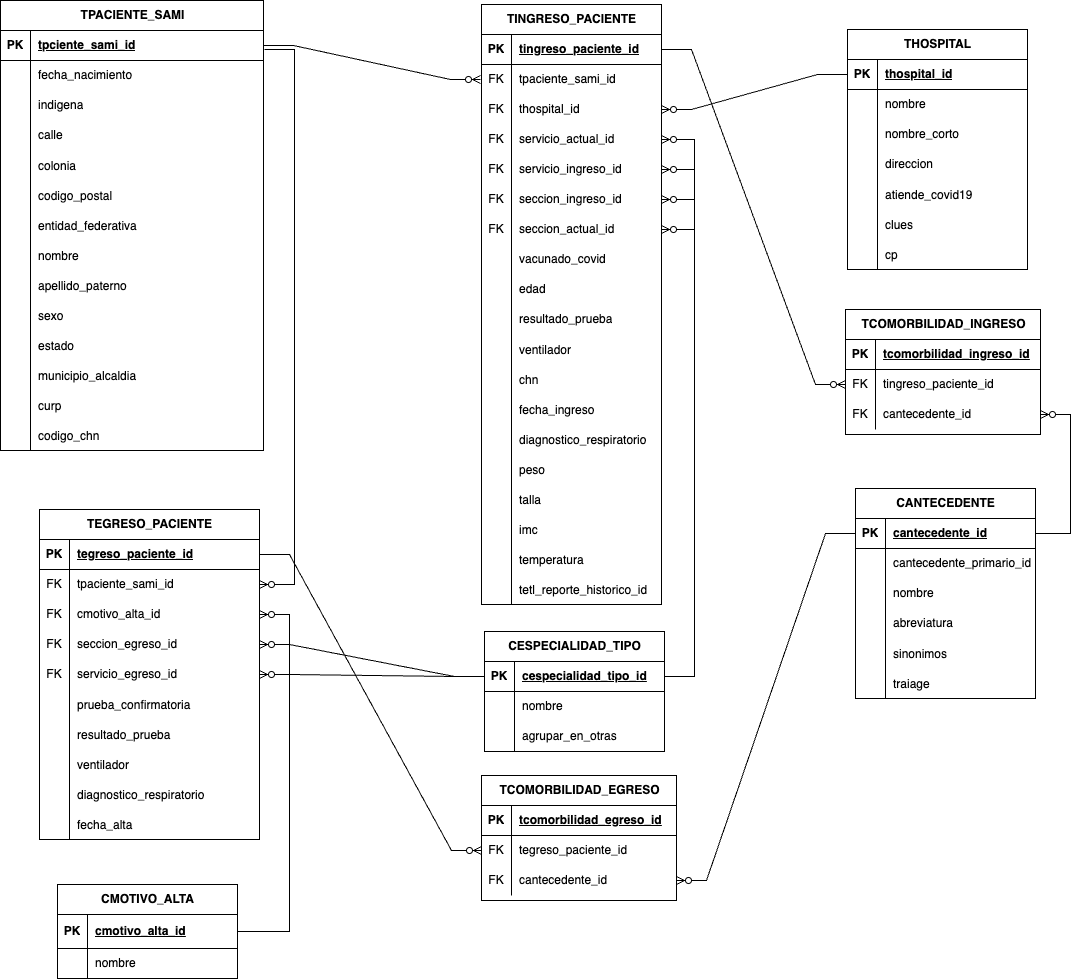
\includegraphics[width=0.9\textwidth]{images/diagrama_er_dashboard.png}
        \caption{Diagrama Entidad-Relación que muestra como se relacionan las tablas usadas para el desarrollo del tablero de datos.} \label{fig:diagramaER_proyecto}
\end{figure}

\newpage

\section{Arquitectura de la aplicación web}



La aplicación web cuenta con una interfaz gráfica desarrollada con React 18 para darle un dinamismo de última generación al Frontend, mientras que el Backend está desarrollado con Django 3 para:

\begin{enumerate}
    \item Poder integrar algoritmos de Machine Learning, Natural Language Processing y todo lo que se pueda requerir y de lo cual se provee mediante Python.
    \item Tener un manejo sencillo y seguro de autenticación.
    \item Armar una estructura cómoda e inteligible de modelos.
    \item Y finalmente, para tener una forma sencilla de conectarnos con el Frontend por medio de Django Rest Framework al crear endpoints de comunicación.
\end{enumerate}

La integración entre React y Django se realiza a través de solicitudes HTTP y respuestas de API REST. React realiza solicitudes a los endpoints proporcionados por Django para obtener o enviar datos. Esta comunicación bidireccional permite una sincronización efectiva entre el frontend y el backend, asegurando una experiencia de usuario sin interrupciones. En la Figura \ref{fig:arquitectura_app} se representa el flujo de procesos que sigue la arquitectura de la aplicación web.



\begin{figure}[H]
        \centering
        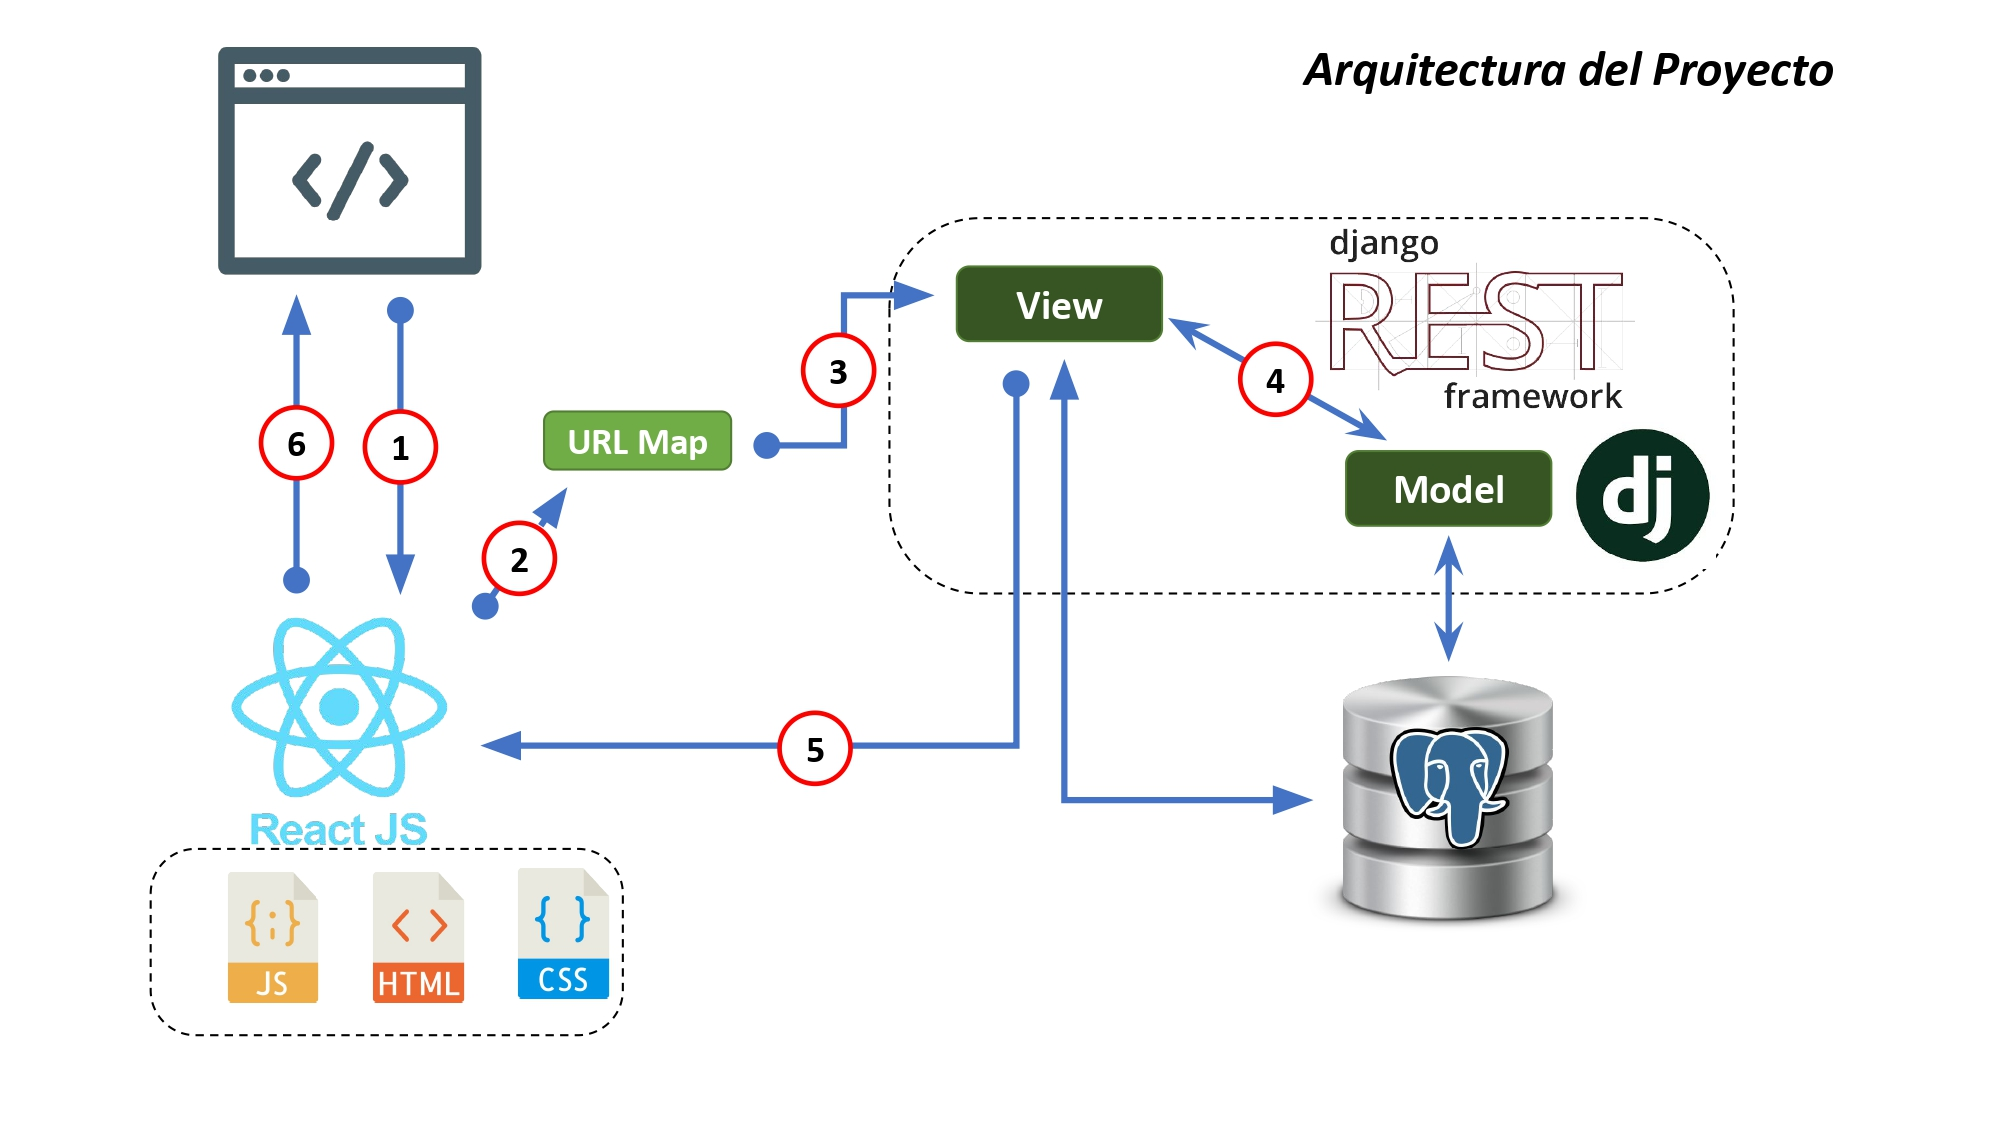
\includegraphics[width=0.8\textwidth]{images/arquitectura_app.jpg}
        \caption{Diagrama de flujo de la arquitectura implementada en la aplicación web.} \label{fig:arquitectura_app}
\end{figure}

La manera en la que funciona la aplicación cada vez que se recibe una petición es la siguiente:

\begin{enumerate}
  \item El navegador manda una solicitud.
  \item El \texttt{URLConf} de Django (Django utiliza el URLConf para asociar patrones de URL con funciones o clases de vistas específicas que manejan las solicitudes correspondientes) interpreta la solicitud y ubica a la vista apropiada de la API.
  \item Se envían los datos hacia la petición de la API correspondiente.
  \item La vista interactúa con la base de datos para obtener datos a través de los endpoints.
  \item La vista envía los resultados de la petición.
  \item La plantilla renderiza la respuesta a la solicitud del navegador.
\end{enumerate}

\section{Mockup inicial del tablero}

La interfaz gráfica del módulo correspondiente al tablero se diseñó con base en un mockup proporcionado por SEDESA, el cual sirvió como referencia visual para la implementación del frontend. Este mockup, una representación estática de la interfaz final, fue creado con el objetivo de establecer la estructura y el diseño general de la aplicación antes de la implementación real.\\

Durante el proceso de implementación, surgieron preguntas clave en relación con las especificaciones de los datos necesarios para crear los endpoints en el backend. Las gráficas que se mostraban, plantearon interrogantes sobre la naturaleza y la estructura de los datos que se esperaban para poder crear de manera correcta la interfaz de usuario.\\

El módulo a desarrollar consta de 6 páginas.
Cada una de las páginas corresponde a una sección del reporte.\\

Una de las principales incógnitas al inicio del desarrollo fue aclarar si el tablero debía mostrar únicamente datos del día actual o si debía ser flexible para mostrar datos dado un periodo de tiempo seleccionado por el usuario, como respuesta final, SEDESA solicitó que se pudiera mostrar datos dado un cierto periodo de tiempo, pero que al ingresar al módulo se muestre inicialmente los datos del día en curso.

\subsection{Página 1 - Métricas de ingresos}
La primera página contiene 3 elementos que muestran datos sobre ingresos hospitalarios:

\begin{enumerate}
    \item \textbf{Tabla}
    
    En lo que concierne a los datos mostrados en la tabla, se muestran datos por unidad médica. \\
    Por cada una de las unidades se debe mostrar la siguiente información que está organizada por secciones: \textbf{Total General, Pacientes Hospitalizados, Pacientes en Terapia Intermedia, Pacientes en UCIA, Pacientes en Urgencias} y  \textbf{Pacientes que ingresaron y les dieron el alta el mismo día}.\\
    En cada una de estas secciones, se encuentran dos subsecciones: \textit{Ingresos hoy} y \textit{Pacientes que reciben atención}.\\

    Cómo se mencionó, al ingresar por primera vez a este módulo se despliega la información del día en curso, sin embargo el usuario podrá seleccionar el rango de tiempo que se quiera inspeccionar.
     
    \item \textbf{Gráfica pastel}

    En esta gráfica se muestra el porcentaje de pacientes por sexos que ingresaron.
    
    \item \textbf{Gráfica de barras}

    En esta gráfica se muestra el porcentaje correspondiente a pacientes que ingresaron en grupos de edad en intervalos de 10 años.
\end{enumerate}

La Figura \ref{fig:mock_pag1} exhibe la primera página del mockup proporcionado por \textbf{SEDESA}

\begin{figure}[H]
        \centering
        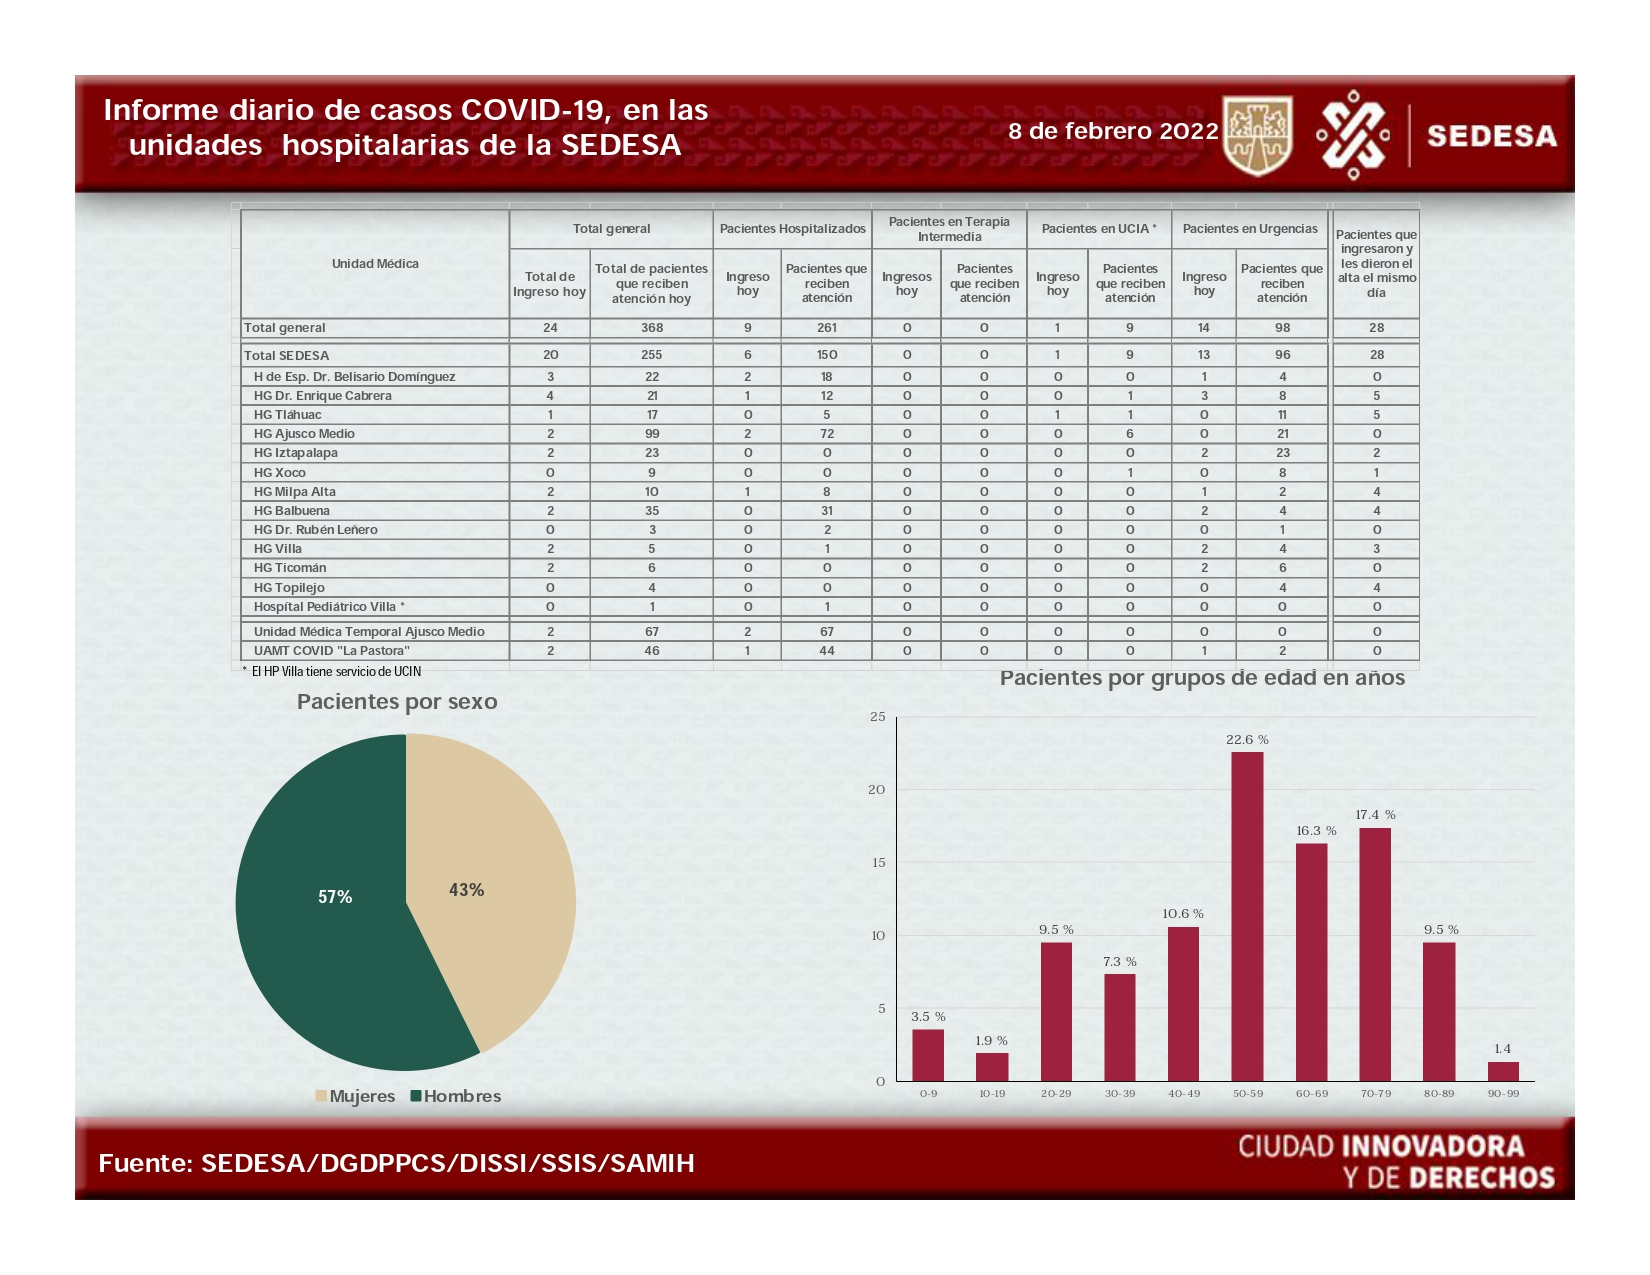
\includegraphics[width=\textwidth]{images/mockup_1.jpg}
        \caption{Página 1 del mockup del tablero de datos.} \label{fig:mock_pag1}
\end{figure}


\subsection{Página 2 - Métricas de egresos}

La segunda página tiene similitudes a la primera, siendo el diferenciador que se muestran métricas correspondientes a los egresos hospitalarios.\\

Contiene 3 elementos que muestran datos sobre los ingresos hospitalarios:

%\newpage

\begin{enumerate}
    \item \textbf{Tabla}
    
    En lo que concierne a los datos mostrados en la tabla, se muestran datos por unidad médica. \\
    Por cada una de las unidades se debe mostrar la siguiente información que está organizada por secciones de acuerdo a que se deben los egresos: \textbf{Total General, Aislamiento en casa, Mejoría, Domicilio, Fuga, Desconocido, Defunciones} y \textbf{Referidos}.\\
    En cada una de estas secciones, se encuentran dos subsecciones: \textit{Hoy} y \textit{Acumulado}.\\

    Esta tabla sigue el mismo comportamiento mencionado de la \textbf{Página 1}.
     
    \item \textbf{Gráfica pastel}

    En esta gráfica se muestra el porcentaje de pacientes por sexos que egresaron.
    
    \item \textbf{Gráfica de barras}

    En esta gráfica se muestra el porcentaje correspondiente a pacientes que egresaron grupos de edad en intervalos de 10.
\end{enumerate}

La Figura \ref{fig:mock_pag2} exhibe la segunda página del mockup proporcionado por \textbf{SEDESA}.

\begin{figure}[H]
        \centering
        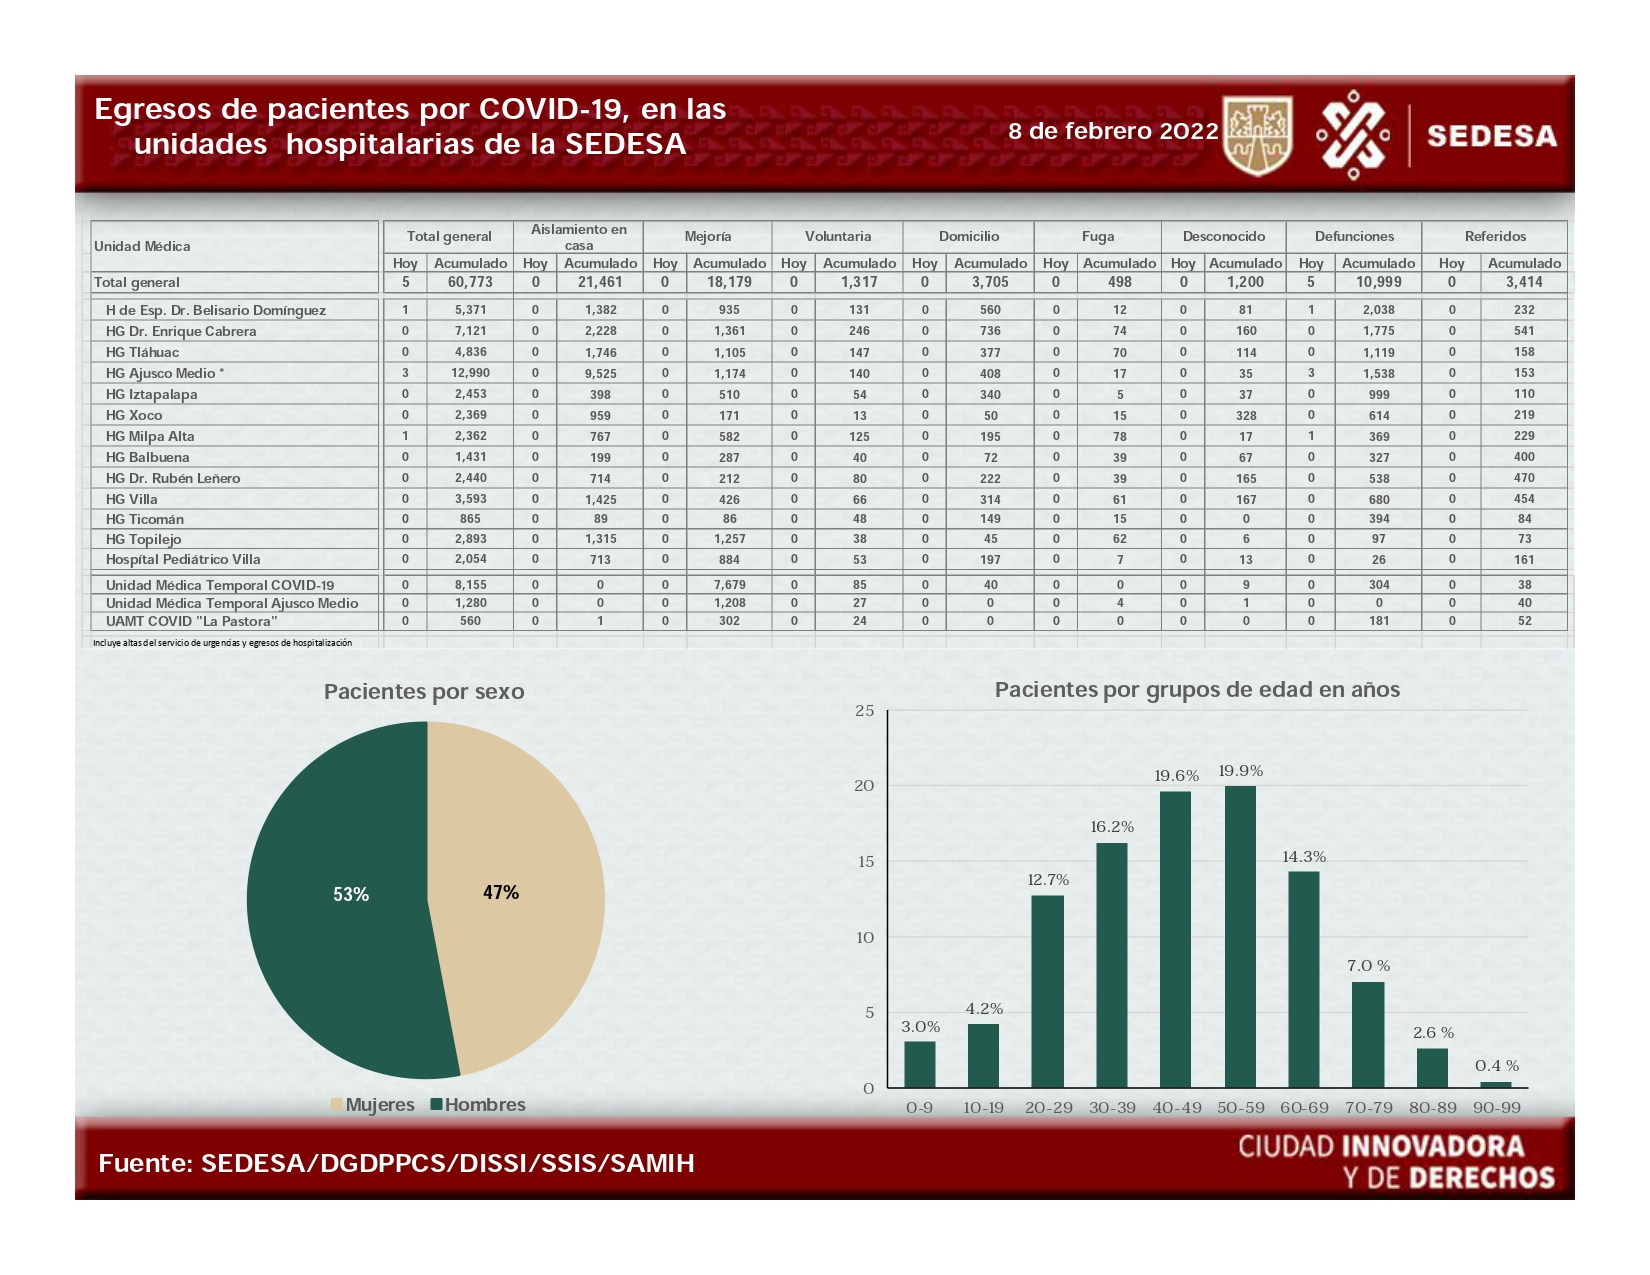
\includegraphics[width=\textwidth]{images/mockup_2.jpg}
        \caption{Página 2 del mockup del tablero de datos.} \label{fig:mock_pag2}
\end{figure}

\subsection{Página 3 - Métricas de defunciones}

En esta página se muestran datos correspondientes a las defunciones registradas en los hospitales de SEDESA.\\

La página cuenta con 3 elementos:

\begin{enumerate}
    \item \textbf{Tabla}\\
    Dentro de esta tabla se mostrarán datos por unidad médica relacionados a defunciones, la tabla distingue hospitales que atienden a pacientes con COVID-19 de los que no.\\
    En su estructura, se incluyen diversas columnas que detallan las defunciones correspondientes al día actual, las acumuladas, las probables a causa del COVID-19 y las confirmadas por esta misma enfermedad.

    \item \textbf{Gráfica de linea}\\
    Esta gráfica muestra las defunciones acumuladas a través del tiempo.

    \item \textbf{Gráfica de barras}\\
    En esta gráfica se muestran el número de defunciones por día.
    
\end{enumerate}

La Figura \ref{fig:mock_pag3} exhibe la tercera página del mockup proporcionado por \textbf{SEDESA}.

\begin{figure}[H]
        \centering
        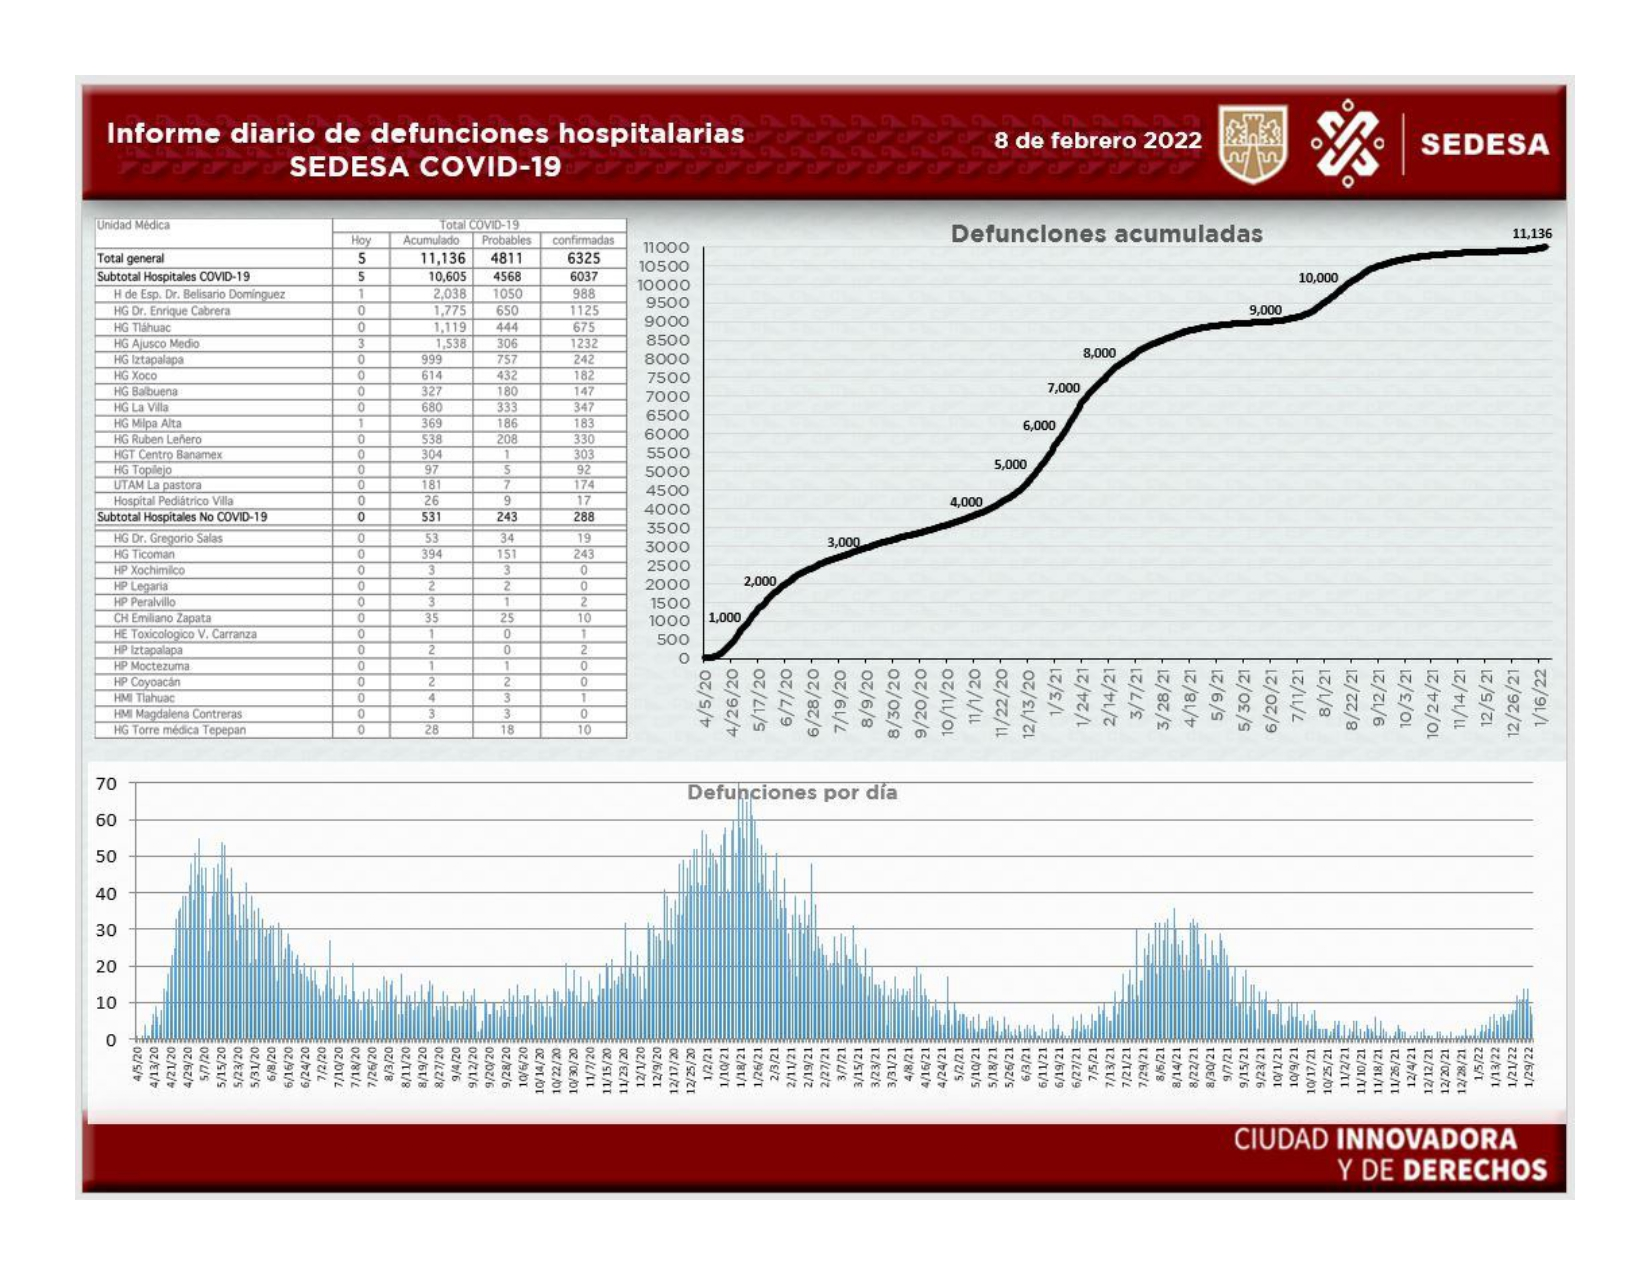
\includegraphics[width=\textwidth]{images/mockup_3.jpg}
        \caption{Página 3 del mockup del tablero de datos.} \label{fig:mock_pag3}
\end{figure}

\subsection{Página 4 - Métricas de defunciones}

Esta página de manera similar a la anterior, muestra más gráficas con datos que hacen referencia a las defunciones.\\

Esta página cuenta con 2 gráficas:

\begin{enumerate}
    \item \textbf{Gráficas de barras}\\
    Esta gráfica muestra el porcentaje de defunciones por grupo de edades quinquenales. 

    \item \textbf{Gráfica de barras empilada}\\
    Esta gráfica muestra el número de defunciones por COVID-19 confirmadas y probables por día de ocurrencia. La particularidad de esta gráfica radica en la disposición de las barras, donde las defunciones confirmadas se superponen a las defunciones probables.
\end{enumerate}

La Figura \ref{fig:mock_pag3} exhibe la cuarta página del mockup proporcionado por \textbf{SEDESA}.

\begin{figure}[H]
        \centering
        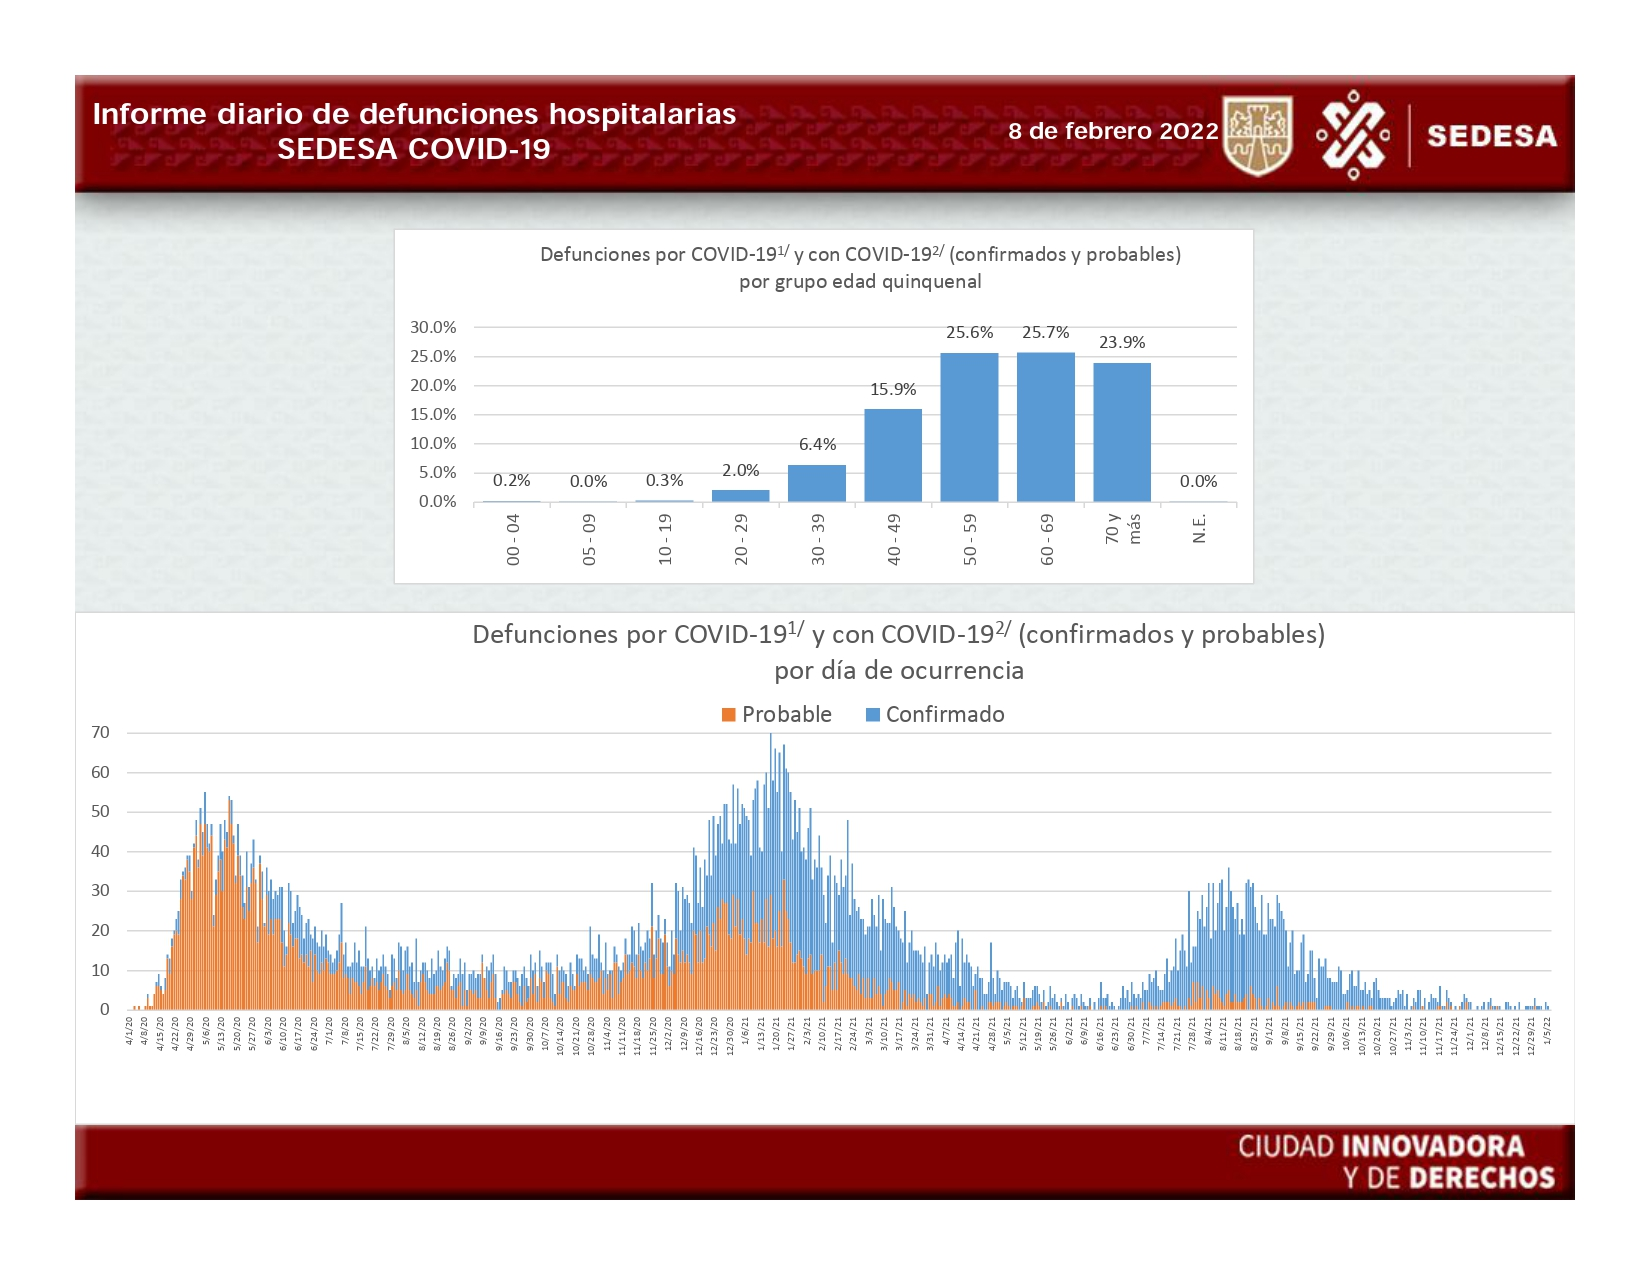
\includegraphics[width=\textwidth]{images/mockup_4.jpg}
        \caption{Página 4 del mockup del tablero de datos.} \label{fig:mock_pag4}
\end{figure}

\subsection{Página 5 - Métricas de defunciones}

Esta página es la última en mostrar gráficas con datos correspondientes a las defunciones.

Se muestran 2 gráficas:

\begin{enumerate}
    \item \textbf{Gráfica pastel}\\
    En esta gráfica se muestra el porcentaje de defunciones por COVID-19 (confirmados y probables) por entidad de residencia habitual.

    \item \textbf{Gráfica de barras}\\
    Esta gráfica expone las defunciones por COVID-19 (confirmados y probables) por año y mes de ocurrencia.
\end{enumerate}

\newpage

La Figura \ref{fig:mock_pag5} exhibe la cuarta página del mockup proporcionado por \textbf{SEDESA}.

\begin{figure}[H]
        \centering
        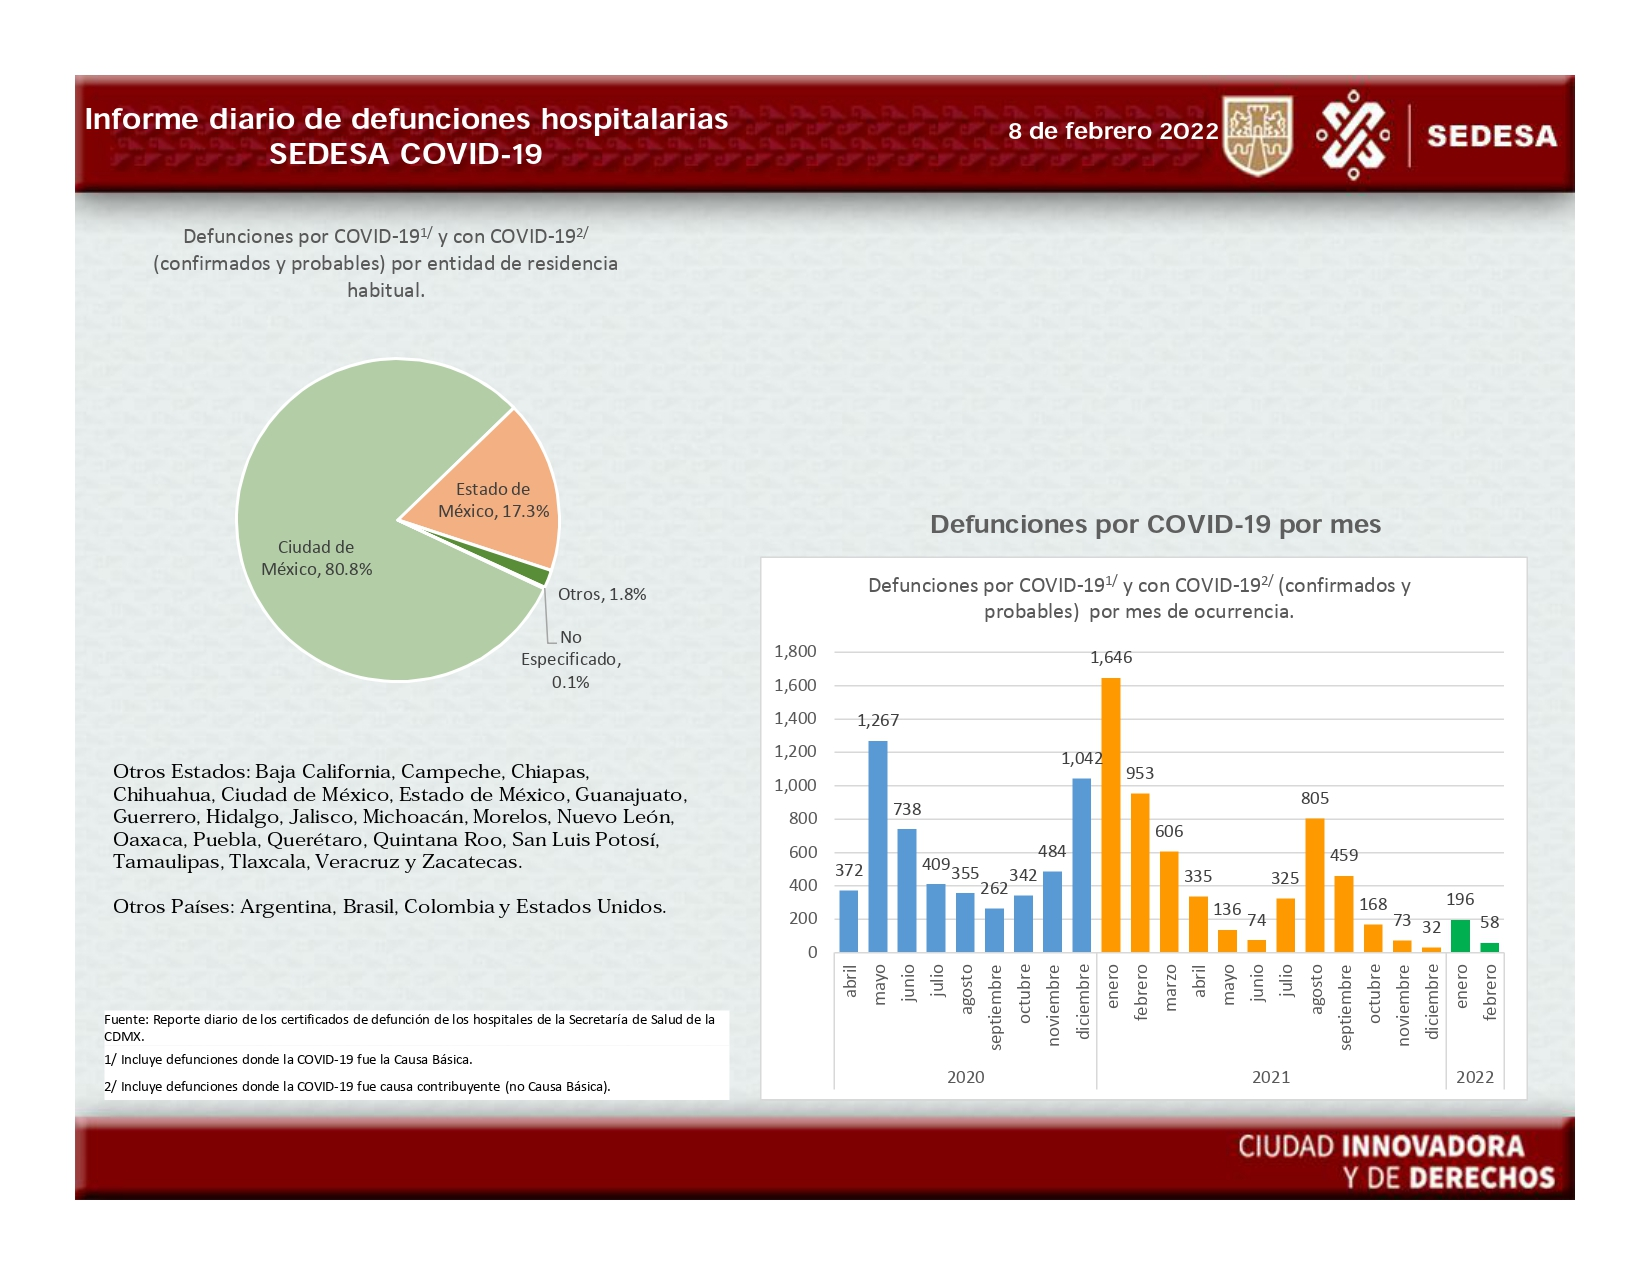
\includegraphics[width=\textwidth]{images/mockup_5.jpg}
        \caption{Página 5 del mockup del tablero de datos.} \label{fig:mock_pag5}
\end{figure}

\subsection{Página 6 - Métricas de traslados}

Como última, esta página muestra datos relacionados a los traslados realizados en los hospitales de SEDESA.

Esta página contiene 4 elementos:

\begin{enumerate}
    \item \textbf{Gráfica de barras 1}\\
    Esta gráfica muestra el número de traslados de pacientes por semana epidemiológica.

    \item \textbf{Gráfica pastel}\\
    Esta gráfica muestra el porcentaje de traslados por sexo.

    \item \textbf{Tabla y gráfica pastel}\\
    En esta tabla y gráfica se muestran datos correspondientes a los traslados por institución.\\

    La tabla muestra el número total de traslados por institución, mientras que la gráfica muestra los datos en términos de porcentaje.

    \item \textbf{Gráfica de barras 2}\\
    En esta gráfica se muestra el número de traslados agrupados por diferentes prioridades: 

    \begin{itemize}
        \item \textbf{R} : Está en riesgo de vida, función y estética.
        \item \textbf{A} : No está en riesgo la vida, función, pero si la estética.
        \item \textbf{V} :  No pone en riesgo la vida, función y estética.
        \item \textbf{N} : Defunción en el lugar.
        \item \textbf{S/D} : Sin dato.
    \end{itemize}
    
\end{enumerate}

La Figura \ref{fig:mock_pag6} exhibe la cuarta página del mockup proporcionado por \textbf{SEDESA}.

\begin{figure}[H]
        \centering
        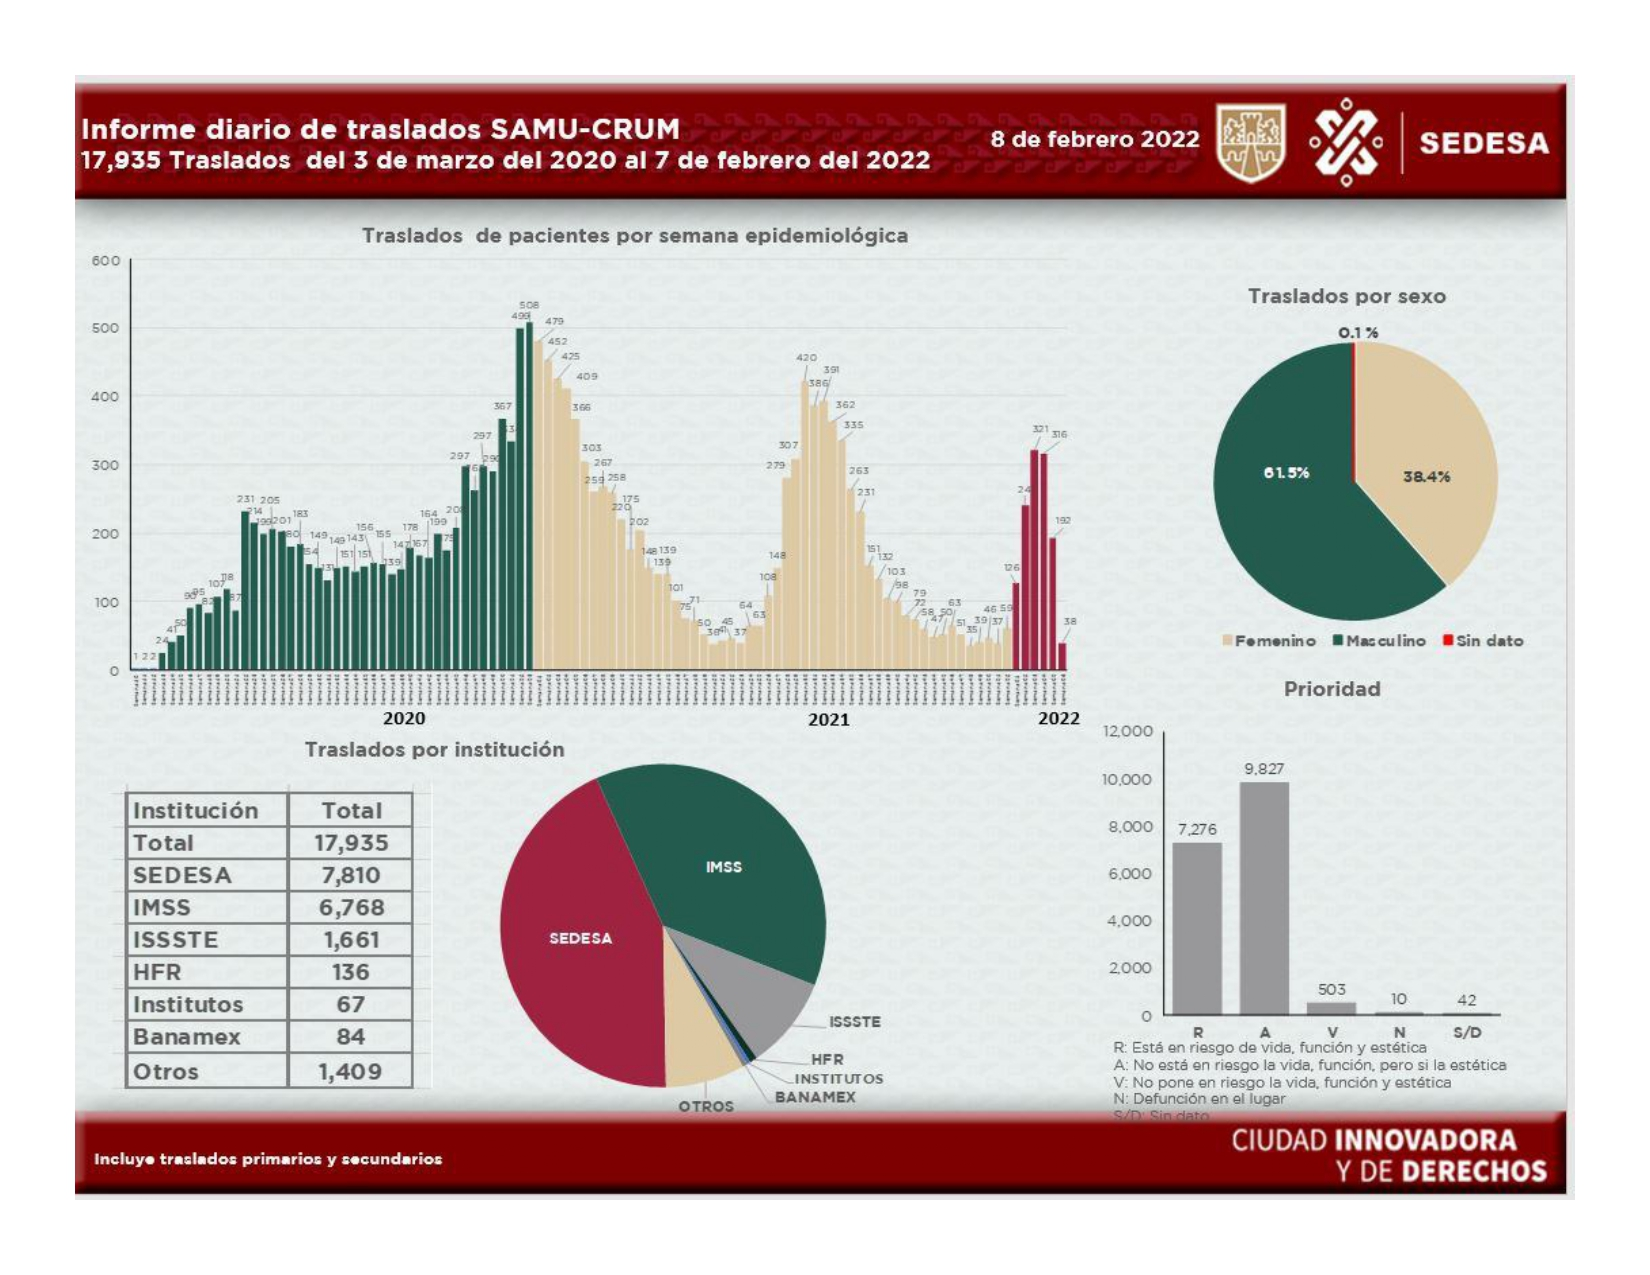
\includegraphics[width=\textwidth]{images/mockup_6.jpg}
        \caption{Página 6 del mockup del tablero de datos.} \label{fig:mock_pag6}
\end{figure}


\section{Backend}\label{sec:backend}

En esta sección, se proporciona una visión detallada del desarrollo del backend del módulo correspondiente al tablero de datos, que abarca la lógica de servidor, la manipulación de datos y la exposición de endpoints a través de Django.\\

Antes de abordar como fue el desarrollo de los endpoints, describiremos de manera breve como está organizado un proyecto en Django.\\

En general, un proyecto en Django está tiene directorios destinados a los diferentes módulos que contenga la aplicación web, en la Figura \ref{fig:backend-estructura} se muestra la estructura en la que está constituida el proyecto.

\begin{figure}
    \dirtree{%
        .1 backend/.
        .2 config/.
        .3 wsgi.py.
        .3 settings.py.
        .3 urls.py.
        .3 decorators.py.
        .2 tableros/.
        .3 migrations/.
        .3 admin.py.
        .3 apps.py.
        .3 models.py.
        .3 tests.py.
        .3 views.py.
        .2 utils/.
        .3 inc\_db.py.
        .3 inc\_utils.py.
        .2 manage.py.
        .2 requirements.txt.
        }
    \caption{Estructura del backend de SI-SEDESA}
    \label{fig:backend-estructura}
\end{figure}

\begin{itemize}[]
  \item \textbf{config/}: Contiene la configuración principal del proyecto.
  \begin{itemize}[]
    \item \textbf{wsgi.py}: Archivo de configuración para el servidor WSGI (Web Server Gateway Interface).
    \item \textbf{settings.py}: Archivo de configuración principal del proyecto.
    \item \textbf{urls.py}: Archivo que contiene las rutas del proyecto.
    \item \textbf{decorators.py}: Archivo con funciones decoradoras para vistas.
  \end{itemize}

  \item \textbf{tableros/}: Directorio del módulo "tableros" que se usó para el tablero de datos.
  \begin{itemize}
    \item \textbf{migrations/}: Directorio que almacena las migraciones de la base de datos.
    \item \textbf{admin.py}: Archivo de registro de modelos para el panel de administración.
    \item \textbf{apps.py}: Archivo de configuración de la aplicación.
    \item \textbf{models.py}: Archivo donde se definen los modelos de datos (tablas de la base de datos).
    \item \textbf{tests.py}: Archivo con pruebas unitarias para la aplicación.
    \item \textbf{views.py}: Archivo que contiene las funciones de vista (views), es decir los endpoints.
    \item \textbf{urls.py}: Archivo que se utiliza para definir las URL de los endpoints del módulo y cómo deben ser manejadas. 
  \end{itemize}

  \item \textbf{utils/}: En este directorio se encuentran archivos que contiene clases y funciones auxiliares para la manipulación de datos y conexión a la base de datos.

  \begin{itemize}
      \item \textbf{inc\_db.py}: Archivo que contiene una clase que se encarga de todas las interacciones directas con la base de datos. La clase posee métodos que sirven para abrir o cerrar la conexión con la base de datos, inserción, actualización, ejecución de consultas y eliminación de registros.

      \item \textbf{inc\_utils.py}: Archivo que contiene funciones genéricas que pueden ser utilizadas en cualquier parte del backend.
  \end{itemize}
  
  \item \textbf{manage.py}: Script de gestión del proyecto.

  \item \textbf{requirements.txt}: Archivo que lista las dependencias y versiones de las bibliotecas utilizadas.\\
\end{itemize}

En especifico, para el desarrollo de este trabajo sólo se trabajó con los archivos \texttt{views.py} y \texttt{urls.py} dentro del directorio \textbf{tableros/}. \\
Cabe mencionar que dentro del directorio de \textbf{backend/} existen más directorios correspondientes a los módulos de la aplicación, los cuales quedan fuera del alcance de este trabajo.


\subsection{Vistas en Django}
Dentro de Django, las vistas son componentes clave que gestionan la lógica detrás de un endpoint específico. Pueden ser funciones o clases, y se encargan de procesar la solicitud HTTP y generar una respuesta. En nuestro caso en particular se crearon únicamente funciones.

Cuando se realiza una solicitud HTTP a un endpoint específico, Django sigue un flujo predefinido para manejar esa solicitud mediante una vista:

\begin{enumerate}
    \item \textbf{Ruta de URL}\\
    La ruta de URL proporcionada en la solicitud se compara con las definiciones de URL en el archivo \texttt{urls.py} de la aplicación para determinar qué vista debe manejar la solicitud.

    \item \textbf{Llamada a la Vista}\\
    La vista asociada a la ruta de URL se llama con la solicitud como argumento.

    \item \textbf{Procesamiento de la solicitud}\\ La vista procesa la solicitud, realiza operaciones necesarias (consultas a la base de datos, manipulación de datos, etc.) y prepara una respuesta.

    \item \textbf{Generación de la respuesta}\\
    La vista devuelve una respuesta, que puede ser un objeto \texttt{Response}, un objeto \texttt{JsonResponse}, o la renderización de una plantilla. En nuestro proyecto regresamos un objeto \texttt{Response}.

    \item \textbf{Envío de la respuesta}\\
    La respuesta se envía al cliente que realizó la solicitud.

\end{enumerate}

\subsection{Estructura de endpoints}

Antes de en listar los endpoints creados para el tablero de datos, se mostrará la lógica y estructura con la que se programaron.\\

Como se mencionó en la sección de la \textbf{Arquitectura de la aplicación web} el backend recibe peticiones mandadas a través del navegador (frontend) cuando un usuario realiza alguna acción que modifique el estado del tablero.\\

La Figura \ref{fig:estructura-peticion} muestra los datos que contienen las peticiones.
\begin{figure}[H]
    \centering
    \begin{lstlisting}[language=json, style=json]
    {
      token: <Token que valida que el usuario tiene permisos de acceder al endpoint>,
      fecha_inicio: <Fecha de inicio que se usa como parametro para las consultas>,
      fecha_fin: <Fecha de fin que se usa como parametro para las consultas>,
      usuario_id: <Id del usuario>,
      id_hospital_user: <Id del usuario dentro del hospital al que pertenece>,
      admin: <Indica si el usuario tiene permisos de administrador>
    }
    \end{lstlisting}
    \caption{Estructura de una petición hacia el backend en el módulo de tableros}
    \label{fig:estructura-peticion}
\end{figure}

En especifico para los endpoints, se usan los parámetros \texttt{fecha\_inicio} y \texttt{fecha\_fin} para obtener datos dado un cierto rango de tiempo, si es que estos parámetros no son nulos.\\

Para el desarrollo de los endpoints se apoyó en bibliotecas adicionales para la manipulación de datos: \textit{Pandas, NumPy} y \textit{Regex}. De igual manera se usaron funciones que ya están integradas con el framework de Django.\\
A pesar de que Django incluye un sistema de modelos que se definen en el archivo \texttt{models.py} los cuales se puede usar para realizar consultas a la base de datos sin la necesidad de escribir las consultas en SQL únicamente, para este proyecto se optó por si realizar todas las consultas hacía la base de datos mediante SQL para que en caso de tener que hacer modificaciones a los endpoints en el futuro, sea más flexible.\\

Ahora, se verá la lógica que siguen todos los endpoints creeados, tomando como ejemplo el endpoint \texttt{get\_traslados\_por\_sexo}. Este endpoint tiene como objetivo proporcionar datos sobre el número total de traslados de pacientes según el sexo, dentro de un rango de fechas especificado. Se listarán los pasos que sigue la lógica de este endpoint, desde la validación de permisos y la obtención de parámetros de fecha hasta la construcción de consultas SQL dinámicas y la preparación de respuestas de la API.\\

\begin{minted}[
frame=lines,
framesep=2mm,
bgcolor=LightGray,
fontsize=\scriptsize,
linenos
]{python}
@api_view(['GET', 'POST'])
@validate_token_permission(url='tablero', acciones_a_validar=['listar'])
def get_traslados_por_sexo(request):
    contexto = {}
    try:
        fechaInicio = request.data.get('fecha_inicio')
        fechaFin = request.data.get('fecha_fin')
        
        if fechaInicio == None:
            fechaInicio = 'NULL'
        else:
            fechaInicio = "'" + request.data.get('fecha_inicio') + "'"

        if fechaFin == None:
            fechaFin = 'NULL'
        else:
            fechaFin = "'" + request.data.get('fecha_fin') + "'"
            
        sql = f"""
            SELECT
                COUNT(*) AS total,
                CASE
                    WHEN p.sexo = 'H' THEN 'Hombres'
                    ELSE 'Mujeres'
                END AS sexo
            FROM
                dashboards.tegreso_paciente e
            INNER JOIN
                dashboards.tpaciente_sami p
            ON 
                e.tpaciente_sami_id = p.tpaciente_sami_id 
            WHERE
                (({fechaInicio} IS NULL AND {fechaFin} IS NULL) OR 
                (e.fecha_alta >= {fechaInicio} AND {fechaFin} IS NULL) OR 
                (e.fecha_alta BETWEEN {fechaInicio} AND {fechaFin})) AND
                e.cmotivo_alta_id = 2
            GROUP BY
                2
        """
        pacientes = db.get_all_pandas(sql)
        if not isinstance(pacientes, bool):
            pacientes = pd.DataFrame(pacientes).replace({np.nan: None})

            contexto['totales_generales'] = {
                'total': pacientes['total'].sum(),
                'sexo': 'Sexo correspondiente'
            }

            pacientes = pacientes.to_dict('records')
        elif isinstance(pacientes, bool):
            print("Error de consulta:\n{}".format(db.error))
            contexto['log'] = "Error de consulta: {}".format(db.error)
            contexto['error'] = 'No existen datos de Pacientes'
            return Response(contexto, status=status.HTTP_400_BAD_REQUEST)

        contexto['pacientes'] = pacientes
        return Response(contexto, status=status.HTTP_200_OK)

    except:
        echo_error(contexto, traceback.format_exc().replace('\n', ' '), 
        'get_traslados_por_sexo')
        return Response(contexto, status=status.HTTP_400_BAD_REQUEST)
\end{minted}


\begin{enumerate}
    \item \textbf{Validación de permisos y token}:
    
       Se realiza una validación del token de autenticación y los permisos del usuario para garantizar que tenga autorización para acceder a esta funcionalidad, en este caso, la acción de listar datos del tablero. Para esto se usa el decorador \texttt{validate\_token\_permission} definido en \textbf{config/decorators.py}, y el decorador \texttt{api\_view} que viene incluido con Django.
    
    \item \textbf{Obtención de parámetros de fecha}:
    
        Se obtienen los parámetros de fecha de inicio y fecha fin de la solicitud (\texttt{request}). Estos parámetros son opcionales y se utilizan para filtrar los datos dado un intervalo de fechas. En caso de ser nulas, se obtendrán todos los datos disponibles.
    
    \item \textbf{Construcción y ejecución de la consulta SQL}:
   
   Se construye una consulta SQL dinámica utilizando los parámetros de fecha obtenidos de la solicitud. Se manejan casos en los que los parámetros de fecha pueden ser nulos, asignándoles el valor \texttt{NULL} en la consulta SQL. Posteriormente, se ejecuta la consulta SQL creada usando la varibale \texttt{db} que es una instancia de la clase que se encarga de todas las intereacciones con la base de datos definida en \textbf{utilis/inc\_db.py}.

    

    \item \textbf{Procesamiento de los resultados}:
    
     Se procesan los resultados de la consulta SQL. Si la consulta se ejecuta correctamente y devuelve datos, se prepara una respuesta con los resultados. Cabe mencionar que hay ciertos endpoints en los cuales se usan las bibliotecas de manipulación de datos anteriormente mencionadas para realizar algún tipo de procesamiento posterior.\\
        En caso de que la consulta no devuelva datos, se registra un mensaje de error y se devuelve una respuesta indicando que no hay datos disponibles.
    
    \item \textbf{Respuesta de la API}:
    
   Finalmente, se envía una respuesta HTTP al cliente, que incluye los datos solicitados y cualquier mensaje de error en caso de que ocurra algún problema durante el procesamiento de la solicitud.\\

   En la Figura \ref{fig:json-estructura} se muestra la estructura de la respuesta que se manda al frontend.

   \begin{figure}[H]
    \centering
    \begin{lstlisting}[language=json, style=json]
    {
      "totales_generales": {
        "total": <Numero total de traslados de pacientes>,
        "sexo": "Sexo correspondiente"
      },
      "pacientes": [
        {
          "total": <Numero total de traslados de pacientes de un sexo especifico>,
          "sexo": "<Sexo del paciente>"
        },
        {
          "total": <Numero total de traslados de pacientes de otro sexo especifico>,
          "sexo": "<Sexo del paciente>"
        }
      ]
    }
    \end{lstlisting}
    \caption{Estructura del JSON enviado al frontend}
    \label{fig:json-estructura}
\end{figure}

Como se puede observar, en la llave \texttt{totales\_generales} se da la información general de los datos obtenidos, mientras que en la llave \texttt{pacientes} se provee los datos obtenidos a partir de la consulta de SQL.

\end{enumerate}

\subsection{Endpoints desarrollados para el tablero de datos}
Una vez explicado la lógica y estructura detrás de la implementación de los endpoints, se mencionarán los endpoints creados para el tablero.\\

En la sección dónde se inspeccionó el mockup inicial, se enlistaron y describieron todas las gráficas y tablas. De manera similar, se enlistarán los endpoints correspondientes a cada una las páginas del mockup.

\subsection{Endpoints - Página 1}
\begin{itemize}
    \item \texttt{get\_info\_detallada\_ingresos}\\
    En este endpoint se obtiene la información para la tabla dónde se muestran datos de ingresos por unidad médica.

    \item \texttt{get\_pacientes\_por\_sexo\_egreso}\\
    En este endpoint se obtiene la información para la gráfica pastel que muestra el porcentaje de pacientes ingresados agrupado por sexos.

    \item \texttt{get\_pacientes\_por\_grupo\_edad}\\
    En este endpoint se obtiene la información para la gráfica de barras que muestra el porcentaje de pacientes ingresados agrupados por grupos de edad.
    
\end{itemize}

\subsection{Endpoints - Página 2}
\begin{itemize}
    \item \texttt{get\_info\_detallada\_ingresos}\\
    En este endpoint se obtiene la información para la tabla dónde se muestran datos de ingresos por unidad médica.

    \item \texttt{get\_pacientes\_por\_sexo\_egreso}\\
    En este endpoint se obtiene la información para la gráfica pastel que muestra el porcentaje de pacientes ingresados agrupado por sexos.

    \item \texttt{get\_pacientes\_por\_grupo\_edad}\\
    En este endpoint se obtiene la información para la gráfica de barras que muestra el porcentaje de pacientes ingresados agrupados por grupos de edad.
    
\end{itemize}

\subsection{Endpoints - Página 3}
\begin{itemize}
    \item \texttt{get\_defunciones\_diarias}\\
    En este endpoint se obtiene la información para la gráfica de barras que muestra las defunciones diarias por COVID-19 y para la gráfica de linea que muestra el conteo acumulativo de las defunciones.

    \item \texttt{get\_defunciones\_covid19\_por\_unidad\_hospitalaria}\\
    En este endpoint se obtiene la información para la tabla que muestra información de defunciones por COVID-19 agrupadas por unidades hospitalarias.
    
\end{itemize}

\subsection{Endpoints - Página 4}
\begin{itemize}
    \item \texttt{get\_defunciones\_covid\_grupos\_edad}\\
    En este endpoint se obtiene la información para la gráfica de barras que muestra las defunciones por COVID-19 por grupos de edad quinquenales.

    \item \texttt{get\_defunciones\_covid\_por\_dia}\\
    En este endpoint se obtiene la información para la gráfica de barras empilada que despliega las defunciones confirmadas y probables por COVID-19.
    
\end{itemize}

\subsection{Endpoints - Página 5}
\begin{itemize}
    \item \texttt{get\_defunciones\_covid\_por\_entidad}\\
    En este endpoint se obtiene la información para la gráfica pastel que muestra por porcentajes las defunciones por COVID-19 por entidad de residencia.

    \item \texttt{get\_defunciones\_covid\_por\_mes}\\
    En este endpoint se obtiene la información para la gráfica de barras que muestra las defunciones por COVID-19 agrupadas por mes y año.
    
\end{itemize}

\subsection{Endpoints - Página 6}
\begin{itemize}
    \item \texttt{get\_traslados\_semama\_epidemiologica}\\
    En este endpoint se obtiene la información para la gráfica de barras que muestra el número de traslados por semana epidemiológica.

    \item \texttt{get\_traslados\_por\_prioridad}\\
    En este endpoint se obtiene la información para la gráfica de barras que muestra el número de traslados por tipo de prioridad.

    \item \texttt{get\_traslados\_por\_sexo}\\
    En este endpoint se obtiene la información para la gráfica pastel que muestra el porcentaje de traslados por sexo.

    \item \texttt{get\_traslados\_por\_institucion}\\
    En este endpoint se obtiene la información para la gráfica pastel y la tabla que muestra el número de traslados agrupados por institución.
\end{itemize}

\section{Frontend}\label{sec:frontent}
En cuanto a la parte del frontend del proyecto, como se mencionó está implementando a través de ReactJS y en especifico para el módulo correspondiente al tablero de datos se utilizó la biblioteca AmCharts para encargarse de todo lo relacionado a la visualización de datos.\\

De manera similar como se hizo en la sección anterior, en la Figura \ref{fig:frontend-estructura} se ilustra como está organizado los directorios en los cuales se trabajó en el frontend:

\begin{figure}[H]
    \dirtree{%
        .1 frontend/.
        .2 src/.
        .3 api/.
        .3 components/.
        .4 tableros/.
        .5 Cards/.
        .5 Charts/.
        .5 DataTables/.
        .3 css/.
        .3 pages/.
        .4 tableros/.
        .2 package-lock.json.
        }
    \caption{Estructura del frontend de SI-SEDESA}
    \label{fig:frontend-estructura}
\end{figure}

\begin{itemize}
    \item \texttt{src/}: Directorio principal donde se encuentra todo el código fuente de la aplicación frontend.
    \begin{itemize}
        \item \texttt{api/}: Directorio que contiene archivos de cada módulo del proyecto para poder hacer peticiones a los endpoints del backend.
        \item \texttt{components/}: Contiene componentes correspondientes a cada uno de los módulos del proyecto.
            \begin{itemize}
                \item \texttt{tableros/}: Específicamente, este directorio contiene todos los componentes relacionados con el tablero de datos.
                    \begin{itemize}
                        \item \texttt{Cards/}: Este directorio contiene los componentes relacionados a las 6 páginas que componen el tablero de datos.
                        \item \texttt{Charts/}: Este directorio contiene componentes reusables para la visualización de datos como gráficas y tablas.

                        \item \texttt{DataTables/}: Este directorio contiene JSON correspondientes a las estructura las tablas que se despliegan en el tablero.
                    \end{itemize}
            \end{itemize}
        \item \texttt{css/}: Contiene archivos CSS para estilos específicos de la aplicación.
        \item \texttt{pages/}: Contiene los archivos principales de cada de uno de los módulos.
            \begin{itemize}
                \item \texttt{tableros/}: Específicamente, este directorio contiene los archivos correspondientes a los tableros que muestran en la aplicación, incluyendo el desarrollado en este trabajo.
            \end{itemize}
    \end{itemize}

    \item \texttt{package-lock.json}: Este es un archivo generado automáticamente por el manejador de paquetes \textit{npm} que utiliza la aplicación, aquí se mantiene un registro detallado y preciso de las versiones de las dependencias que se utilizan y que deberán ser instaladas.
\end{itemize}

Para el caso particular del tablero de datos se trabajaron en los siguientes archivos:

\begin{enumerate}
    \item \texttt{api/tableros.jsx}

    En este archivo se definieron todas las llamadas hacia cada uno de los endpoints, para esto se hizo de la biblioteca de \textbf{axios} que se utiliza para realizar solicitudes HTTP desde el navegador. \\

    A continuación se muestra un ejemplo de como se programaron funciones para hacer peticiones a los endpoints y directorios:

    \begin{minted}[
    frame=lines,
    framesep=2mm,
    bgcolor=LightGray,
    fontsize=\scriptsize,
    linenos
    ]{js}
    export const get_traslados_por_sexo = (auth, startDate, endDate) => {
      try {
        const response = axios({
          method: "POST",
          baseUrl: BASE_URL,
          url: FORM_URL_TRASLADOS_POR_SEXO,
          headers: {
            Accept: "application/json",
            "Content-Type": "application/json",
            "X-CSRFToken": cookies.get("csrftoken"),
            Authorization: `Bearer ${auth.token}`,
          },
          withCredentials: true,
          data: { token: auth.token,
            fecha_inicio: startDate,
            fecha_fin : endDate
           },
        });
        return response; 
      } catch (error) {
      }
    };
    \end{minted}
Este código define una función llamada \texttt{get\_traslados\_por\_prioridad} que realiza una petición a un endpoint \textbf{get\_tralados\_por\_prioridad} definido anteriormente en el backend, utilizando \textbf{axios} para realizar solicitudes HTTP. \\
Los aspectos a destacar son los siguientes:
\begin{itemize}
    \item Configuración de la petición:
    \begin{itemize}
        \item Se utiliza el método POST para enviar la solicitud al servidor.
        \item Se especifica la \texttt{baseUrl} como una variable \texttt{BASE\_URL}, la cual hace referencia a la URL base de la aplicación.
        \item Se establece la URL del endpoint a la que se realizará la petición, utilizando la variable \texttt{FORM\_URL\_TRASLADOS\_POR\_PRIORIDAD} la cual tiene el valor \texttt{'/tableros/get\_traslados\_por\_prioridad/'}. \\
        Cabe mencionar que todos los endpoints relacionados a el tablero de datos tiene el prefijo \texttt{'/tableros/'}
        \item Se definen los encabezados de la solicitud, incluyendo el tipo de contenido esperado y el token de autorización.
        \item Se habilita la opción \texttt{withCredentials} para permitir el envío de cookies en la solicitud.
    \end{itemize}
    \item Datos enviados en la solicitud:
    \begin{itemize}
        \item Se envían al backend los datos en formato JSON que incluyen el token de autenticación (\texttt{auth.token}), la fecha de inicio (\texttt{startDate}) y la fecha de fin (\texttt{endDate}).
    \end{itemize}
\end{itemize}

\item \texttt{components/Charts}

Dentro de este directorio se definieron todos los componentes que corresponden a cada una de las gráficas que deben mostrarse. Para ello se crearon los siguientes archivos:

\begin{itemize}
    \item \texttt{BarChart.jsx}

    Este archivo corresponde a la implementación y definición de una gráfica de barras tradicional.
    
    \item \texttt{BarChartCategory.jsx}

    Este archivo corresponde a la implementación y definición de una gráfica de barras la cual agrupa los datos mediante categorías.
    
    \item \texttt{LineChart.jsx}

    Este archivo corresponde a la implementación y definición de una gráfica de linea que muestra datos a lo largo de una línea continua.
    
    \item \texttt{MonthlyBarChart.jsx}

    Este archivo corresponde a la implementación y definición de una gráfica de barras la cual agrupa los datos por meses.
    
    \item \texttt{PieChart.jsx}

    Este archivo corresponde a la implementación y definición de una gráfica pastel para mostrar datos en términos de porcentajes.
    
    \item \texttt{StackedBarChart.jsx}

    Este archivo corresponde a la implementación y definición de una gráfica de barras apiladas, donde las barras se superponen para mostrar la contribución de múltiples categorías a un total.
\end{itemize}

A continuación se muestra el código correspondiente a \texttt{LineChart.jsx}, el cual es similar a el código de los demás componentes:

\begin{minted}[
    frame=lines,
    framesep=2mm,
    bgcolor=LightGray,
    fontsize=\scriptsize,
    linenos
    ]{js}
const LineChart = ({ id_chart, textTitle, dataChart = [], titleY, titleX, maxSizeY }) => {

  const chartID = id_chart;

  useLayoutEffect(() => {

    // Inicialización de la gráfica
    let root = am5.Root.new(chartID);

    root.setThemes([
      am5themes_Animated.new(root)
    ]);

    let chart = root.container.children.push(am5xy.XYChart.new(root, {
      panX: true,
      panY: true,
      wheelX: "panX",
      wheelY: "zoomX",
      pinchZoomX:true
    }));

    // Posicionamiento y configuraciones del Titulo
    chart.children.unshift(am5.Label.new(root, {
      text: textTitle,
      fontSize: 18,
      fontWeight: "500",
      textAlign: "center",
      x: am5.percent(50),
      y: -2,
      centerX: am5.percent(50),
      paddingTop: 0,
      paddingBottom: 0
    }));

    // Añadir y configurar ejes
    let xAxis = chart.xAxes.push(am5xy.DateAxis.new(root, {
      maxDeviation: 0.2,
      baseInterval: {
        timeUnit: "day",
        count: 1
      },
      renderer: am5xy.AxisRendererX.new(root, {}),
      tooltip: am5.Tooltip.new(root, {})
    }));

    var xRenderer = xAxis.get("renderer");
    xRenderer.labels.template.setAll({
      rotation: -90,
    });
    
    let yAxis = chart.yAxes.push(am5xy.ValueAxis.new(root, {
      min: 0,
      max: maxSizeY,
      renderer: am5xy.AxisRendererY.new(root, {})
    }));

    // Se añaden los datos
    let series = chart.series.push(am5xy.SmoothedXLineSeries.new(root, {
      name: "Series",
      xAxis,
      yAxis,
      valueYField: titleY,
      valueXField: titleX,
      tooltip: am5.Tooltip.new(root, {
        labelText: "{valueY}"
      })
    }));

    xAxis.get("dateFormats")["day"] = "MM/dd/yy";
    series.data.setAll(dataChart);

    let cursor = chart.set("cursor", am5xy.XYCursor.new(root, {
      behavior: "none"
    }));
    cursor.lineY.set("visible", false);

    chart.set("scrollbarX", am5.Scrollbar.new(root, {
      orientation: "horizontal"
    }));

    xAxis.get("renderer").labels.template.setAll({
      oversizedBehavior: "wrap",
      textAlign: "center",
      maxWidth: 150
    });

    series.appear(1000);
    chart.appear(1000, 100);

    return () => root.dispose();
  });
\end{minted}

Este código utiliza la función \texttt{useLayoutEffect} de ReactJS para realizar operaciones de inicialización y configuración de la gráfica cuando el componente se carga por primera vez.
En la gráfica, se establece un título, se configuran los ejes X e Y con sus respectivos títulos y límites, se añaden los datos proporcionados y se configura un cursor interactivo.\\
De una manera similar las gráficas restantes fueron programadas.


\item \texttt{components/Cards}

Dentro de este directorio se definieron todos los componentes que corresponden a cada una de las seis páginas que conforman el tablero: \texttt{Pagina1.jsx}, \texttt{Pagina2.jsx}, \texttt{Pagina3.jsx}, \texttt{Pagina3.jsx}, \texttt{Pagina5.jsx} y \texttt{Pagina6.jsx}.
\\

La estructura de cada uno de estos archivos es similar, lo que difiere es la forma en que se estructura el código HTML de acuerdo a como debem posicionados cada uno de los elementos. A continuación se muestra el código correspondiente a la página 3:
\\

\begin{minted}[
    frame=lines,
    framesep=2mm,
    bgcolor=LightGray,
    fontsize=\scriptsize,
    linenos
    ]{js}
import React, {useEffect, useState} from 'react';

// Charts
import LineChart from '../Charts/LineChart'
import BarChart from '../Charts/BarChart'

//Api
import {
  get_defunciones_diarias,
  get_defunciones_covid19_por_unidad_hospitalaria
} from '../../../api/tableros';

//Alerts
import { handleError } from '../../../api/error';

//Encabezados de tablas
const tableHeaders15 = require('../DataTables/Table15.json');

function generateRegressionData(data) {
  let modifiedData = [];

  if (data.length === 0){
    return [];
  }

  for (let i = 0; i < data.length; i++) {
    let item = data[i];
    item.acumulated = 0;
    item.date = new Date(item.fecha_alta).getTime();
    modifiedData.push(item);
  }

  modifiedData[0].acumulated = modifiedData[0].total;

  for (let i = 1; i < data.length; ++i) {
    modifiedData[i].acumulated = modifiedData[i].total + modifiedData[i-1].acumulated;
  }

  return modifiedData;
}

const Pagina3 = ({startDate, endDate}) => {
  const {auth} = useAuth();
  const [barData, setBarData] = useState([]);
  const [tableData, setTableData] = useState([]);

  useEffect(() => {
    const getDataBar = async () => {
      try {
        const {data} = await get_defunciones_diarias(auth, startDate, endDate);
        const modifiedData = generateRegressionData(data.defunciones);
        setBarData(() => modifiedData);
      } catch (error) {
        handleError('Error datos Bar3', error)
      }
    };
    const getTableData = async () => {
      try {
        const {data} = await get_defunciones_covid19_por_unidad_hospitalaria(auth, startDate, 
        endDate);
        setTableData(() => data.defunciones);
      } catch (error) {
        handleError('Error datos Table3', error)
      }
    };
    getDataBar();
    getTableData();
  }, [startDate, endDate]);

  return (
    <div style={{'min-height': '100vh'}}>
      <div className='grid grid-cols-12 gap-12 pt-12'>
      <div className='col-start-2 col-span-4 pt-4'>
          <TableG
            columnDefs={tableHeaders15}
            rowData={tableData}
            heightValue='h-80'/>
      </div>
      <div id='pagina3Defunciones' className='chart col-start-7 col-span-4'>
          <LineChart
            id_chart='pagina3Defunciones'
            textTitle='Defunciones acumuladas'
            dataChart={barData}
            valueField='acumulated'
            dateField='date'/>
        </div>
        <div id='pagina3DefuncionesPorDia' className='chart col-start-3 col-span-8'>
          <BarChart
            id_chart='pagina3DefuncionesPorDia'
            textTitle='Defunciones por día'
            dataChart={barData}
            valueField='total'
            dateField='date'
            />
        </div>
      </div>
      <ListonInf/>
    </div>
  )
};

export default Pagina3
\end{minted}

Se utiliza el hook \texttt{useEffect} para realizar operaciones secundarias después de que la renderización ha ocurrido. Se definen dos funciones, \texttt{getDataBar} y \texttt{getTableData}, que llaman a los endpoints para obtener los datos Una vez que los datos se obtienen con éxito, se actualizan los estados \texttt{barData} y \texttt{tableData} utilizando los métodos \texttt{setBarData} y \texttt{setTableData}. Finalmente, se incluyen \texttt{startDate} y \texttt{endDate} en la lista de dependencias del \texttt{useEffect}, asegurando que estas operaciones se vuelvan a realizar cada vez que estas propiedades cambian.


\item \texttt{pages/tableros/ReporteDiario.jsx}

Como último, este archivo es el que engloba a cada una de las páginas que conforman el tablero de datos. Este componente permite al usuario seleccionar un rango de fechas mediante un calendario y visualizar las gráficas y tabla con los datos correspondientes al período de tiempo seleccionado También ofrece la opción de generar un PDF del informe mostrado. 

\end{enumerate}

%------------------------------------------------------------------
\section{Resumen}
En este capítulo se describió la metodología propuesta con la que se abordó la implementación del tablero de datos.\\

Se describió cada una de las tablas usadas, así como su relación entre ellas para realizar las consultas hacia la base de datos, que posteriormente se usarían dentro del backend para programar cada uno de los endpoints.\\
Se exhibe el diseño inicial propuesto por \textbf{SEDESA} como punto de partida, con el propósito de identificar de manera clara los conjuntos de datos necesarios para su obtención a través de los endpoints correspondientes.

Por último, se describió la arquitectura en la que está basada el proyecto, así como la estructura tanto del backend como del frontend. Se explicó el trabajado realizado en cada uno de los directorios y archivos. Se describió la lógica detrás de cada unos de los componentes del frontend y la estructura que siguen cada uno de los endpoints creados en la parte del backend.



 
